% Options for packages loaded elsewhere
\PassOptionsToPackage{unicode}{hyperref}
\PassOptionsToPackage{hyphens}{url}
\documentclass[
]{article}
\usepackage{xcolor}
\usepackage{amsmath,amssymb}
\setcounter{secnumdepth}{-\maxdimen} % remove section numbering
\usepackage{iftex}
\ifPDFTeX
  \usepackage[T1]{fontenc}
  \usepackage[utf8]{inputenc}
  \usepackage{textcomp} % provide euro and other symbols
\else % if luatex or xetex
  \usepackage{unicode-math} % this also loads fontspec
  \defaultfontfeatures{Scale=MatchLowercase}
  \defaultfontfeatures[\rmfamily]{Ligatures=TeX,Scale=1}
\fi
\usepackage{lmodern}
\ifPDFTeX\else
  % xetex/luatex font selection
\fi
% Use upquote if available, for straight quotes in verbatim environments
\IfFileExists{upquote.sty}{\usepackage{upquote}}{}
\IfFileExists{microtype.sty}{% use microtype if available
  \usepackage[]{microtype}
  \UseMicrotypeSet[protrusion]{basicmath} % disable protrusion for tt fonts
}{}
\makeatletter
\@ifundefined{KOMAClassName}{% if non-KOMA class
  \IfFileExists{parskip.sty}{%
    \usepackage{parskip}
  }{% else
    \setlength{\parindent}{0pt}
    \setlength{\parskip}{6pt plus 2pt minus 1pt}}
}{% if KOMA class
  \KOMAoptions{parskip=half}}
\makeatother
\usepackage{color}
\usepackage{fancyvrb}
\newcommand{\VerbBar}{|}
\newcommand{\VERB}{\Verb[commandchars=\\\{\}]}
\DefineVerbatimEnvironment{Highlighting}{Verbatim}{commandchars=\\\{\}}
% Add ',fontsize=\small' for more characters per line
\newenvironment{Shaded}{}{}
\newcommand{\AlertTok}[1]{\textcolor[rgb]{1.00,0.00,0.00}{\textbf{#1}}}
\newcommand{\AnnotationTok}[1]{\textcolor[rgb]{0.38,0.63,0.69}{\textbf{\textit{#1}}}}
\newcommand{\AttributeTok}[1]{\textcolor[rgb]{0.49,0.56,0.16}{#1}}
\newcommand{\BaseNTok}[1]{\textcolor[rgb]{0.25,0.63,0.44}{#1}}
\newcommand{\BuiltInTok}[1]{\textcolor[rgb]{0.00,0.50,0.00}{#1}}
\newcommand{\CharTok}[1]{\textcolor[rgb]{0.25,0.44,0.63}{#1}}
\newcommand{\CommentTok}[1]{\textcolor[rgb]{0.38,0.63,0.69}{\textit{#1}}}
\newcommand{\CommentVarTok}[1]{\textcolor[rgb]{0.38,0.63,0.69}{\textbf{\textit{#1}}}}
\newcommand{\ConstantTok}[1]{\textcolor[rgb]{0.53,0.00,0.00}{#1}}
\newcommand{\ControlFlowTok}[1]{\textcolor[rgb]{0.00,0.44,0.13}{\textbf{#1}}}
\newcommand{\DataTypeTok}[1]{\textcolor[rgb]{0.56,0.13,0.00}{#1}}
\newcommand{\DecValTok}[1]{\textcolor[rgb]{0.25,0.63,0.44}{#1}}
\newcommand{\DocumentationTok}[1]{\textcolor[rgb]{0.73,0.13,0.13}{\textit{#1}}}
\newcommand{\ErrorTok}[1]{\textcolor[rgb]{1.00,0.00,0.00}{\textbf{#1}}}
\newcommand{\ExtensionTok}[1]{#1}
\newcommand{\FloatTok}[1]{\textcolor[rgb]{0.25,0.63,0.44}{#1}}
\newcommand{\FunctionTok}[1]{\textcolor[rgb]{0.02,0.16,0.49}{#1}}
\newcommand{\ImportTok}[1]{\textcolor[rgb]{0.00,0.50,0.00}{\textbf{#1}}}
\newcommand{\InformationTok}[1]{\textcolor[rgb]{0.38,0.63,0.69}{\textbf{\textit{#1}}}}
\newcommand{\KeywordTok}[1]{\textcolor[rgb]{0.00,0.44,0.13}{\textbf{#1}}}
\newcommand{\NormalTok}[1]{#1}
\newcommand{\OperatorTok}[1]{\textcolor[rgb]{0.40,0.40,0.40}{#1}}
\newcommand{\OtherTok}[1]{\textcolor[rgb]{0.00,0.44,0.13}{#1}}
\newcommand{\PreprocessorTok}[1]{\textcolor[rgb]{0.74,0.48,0.00}{#1}}
\newcommand{\RegionMarkerTok}[1]{#1}
\newcommand{\SpecialCharTok}[1]{\textcolor[rgb]{0.25,0.44,0.63}{#1}}
\newcommand{\SpecialStringTok}[1]{\textcolor[rgb]{0.73,0.40,0.53}{#1}}
\newcommand{\StringTok}[1]{\textcolor[rgb]{0.25,0.44,0.63}{#1}}
\newcommand{\VariableTok}[1]{\textcolor[rgb]{0.10,0.09,0.49}{#1}}
\newcommand{\VerbatimStringTok}[1]{\textcolor[rgb]{0.25,0.44,0.63}{#1}}
\newcommand{\WarningTok}[1]{\textcolor[rgb]{0.38,0.63,0.69}{\textbf{\textit{#1}}}}
\usepackage{longtable,booktabs,array}
\usepackage{calc} % for calculating minipage widths
% Correct order of tables after \paragraph or \subparagraph
\usepackage{etoolbox}
\makeatletter
\patchcmd\longtable{\par}{\if@noskipsec\mbox{}\fi\par}{}{}
\makeatother
% Allow footnotes in longtable head/foot
\IfFileExists{footnotehyper.sty}{\usepackage{footnotehyper}}{\usepackage{footnote}}
\makesavenoteenv{longtable}
\usepackage{graphicx}
\makeatletter
\newsavebox\pandoc@box
\newcommand*\pandocbounded[1]{% scales image to fit in text height/width
  \sbox\pandoc@box{#1}%
  \Gscale@div\@tempa{\textheight}{\dimexpr\ht\pandoc@box+\dp\pandoc@box\relax}%
  \Gscale@div\@tempb{\linewidth}{\wd\pandoc@box}%
  \ifdim\@tempb\p@<\@tempa\p@\let\@tempa\@tempb\fi% select the smaller of both
  \ifdim\@tempa\p@<\p@\scalebox{\@tempa}{\usebox\pandoc@box}%
  \else\usebox{\pandoc@box}%
  \fi%
}
% Set default figure placement to htbp
\def\fps@figure{htbp}
\makeatother
% definitions for citeproc citations
\NewDocumentCommand\citeproctext{}{}
\NewDocumentCommand\citeproc{mm}{%
  \begingroup\def\citeproctext{#2}\cite{#1}\endgroup}
\makeatletter
 % allow citations to break across lines
 \let\@cite@ofmt\@firstofone
 % avoid brackets around text for \cite:
 \def\@biblabel#1{}
 \def\@cite#1#2{{#1\if@tempswa , #2\fi}}
\makeatother
\newlength{\cslhangindent}
\setlength{\cslhangindent}{1.5em}
\newlength{\csllabelwidth}
\setlength{\csllabelwidth}{3em}
\newenvironment{CSLReferences}[2] % #1 hanging-indent, #2 entry-spacing
 {\begin{list}{}{%
  \setlength{\itemindent}{0pt}
  \setlength{\leftmargin}{0pt}
  \setlength{\parsep}{0pt}
  % turn on hanging indent if param 1 is 1
  \ifodd #1
   \setlength{\leftmargin}{\cslhangindent}
   \setlength{\itemindent}{-1\cslhangindent}
  \fi
  % set entry spacing
  \setlength{\itemsep}{#2\baselineskip}}}
 {\end{list}}
\usepackage{calc}
\newcommand{\CSLBlock}[1]{\hfill\break\parbox[t]{\linewidth}{\strut\ignorespaces#1\strut}}
\newcommand{\CSLLeftMargin}[1]{\parbox[t]{\csllabelwidth}{\strut#1\strut}}
\newcommand{\CSLRightInline}[1]{\parbox[t]{\linewidth - \csllabelwidth}{\strut#1\strut}}
\newcommand{\CSLIndent}[1]{\hspace{\cslhangindent}#1}
\setlength{\emergencystretch}{3em} % prevent overfull lines
\providecommand{\tightlist}{%
  \setlength{\itemsep}{0pt}\setlength{\parskip}{0pt}}
\usepackage{bookmark}
\IfFileExists{xurl.sty}{\usepackage{xurl}}{} % add URL line breaks if available
\urlstyle{same}
\hypersetup{
  pdftitle={TRANSFORMANDO APIS EM INTERFACES CONVERSACIONAIS: VALIDAÇÃO DA ABORDAGEM OPENAPI-MCP PARA AGENTES BASEADOS EM IA},
  hidelinks,
  pdfcreator={LaTeX via pandoc}}

\title{\textbf{TRANSFORMANDO APIS EM INTERFACES CONVERSACIONAIS:
VALIDAÇÃO DA ABORDAGEM OPENAPI-MCP PARA AGENTES BASEADOS EM IA}}
\author{}
\date{}

\begin{document}
\maketitle

\textbf{Lucas de Castro Zanoni}\footnote{Graduando em Engenharia de
  software no semestre de 2025-1. E-mail: castro.lucas290@gmail.com}

\textbf{Thyerri Fernandes Mezzari}\footnote{Professor do Centro
  Universitário UniSATC E-mail: thyerri.mezzari@satc.edu.br}

Resumo: Este trabalho apresenta um estudo experimental preliminar de
integração de agentes conversacionais baseados em IA a soluções web
através da especificação OpenAPI combinada com o protocolo Model Context
Protocol (MCP). A pesquisa investiga como especificações OpenAPI podem
ser automaticamente convertidas em servidores MCP, permitindo que
modelos de linguagem de grande escala (LLMs) interajam com sistemas
externos. O estudo envolveu a implementação de uma prova de conceito que
inclui um gerador automático de servidores MCP a partir de
especificações OpenAPI, um cliente de chat capaz de gerenciar múltiplos
servidores MCP simultaneamente, e aplicações de teste para validação da
abordagem. Para garantir uma análise rigorosa e reprodutível, foi
desenvolvida uma interface padronizada e definidos critérios objetivos,
fundamentando-se em referências acadêmicas, guias de segurança,
relatórios de mercado e documentações oficiais de provedores de modelos
de linguagem, assim como testes automatizados \emph{end-to-end}, com
ênfase em métricas de robustez, segurança (incluindo \emph{red teaming}
e injeção de \emph{prompts}) e usabilidade dentro do escopo experimental
definido. Os resultados indicam a viabilidade técnica inicial e eficácia
da integração OpenAPI-MCP nos cenários testados, fornecendo uma análise
fundamentada sobre os benefícios, desafios e limitações desta abordagem
para a integração de agentes conversacionais baseados em IA em sistemas
complexos. A pesquisa estabelece evidências preliminares convincentes
sobre a possibilidade de grandes avanços na facilitação da integração
entre sistemas existentes e LLMs, promovendo maior acessibilidade,
usabilidade e democratização do acesso a tecnologias complexas,
justificando investigações mais aprofundadas para validação em escala
maior.

\textbf{Palavras-chave:} agente conversacional baseado em IA, integração
de sistemas, inteligência artificial, OpenAPI, Model Context Protocol,
segurança, usabilidade.

\section{1 INTRODUÇÃO}\label{introduuxe7uxe3o}

A evolução das interfaces de usuário tem gerado uma diversidade de
padrões de design e usabilidade, resultando frequentemente em barreiras
para a plena acessibilidade e interação dos usuários com os sistemas
digitais. Com o aumento da complexidade do frontend e a multiplicidade
de paradigmas de interação, muitos usuários enfrentam dificuldades
significativas para utilizar efetivamente as funcionalidades oferecidas
pelas soluções web modernas (RAPP et al., 2018) (KOCABALLI et al.,
2019). Nesse contexto, a ascensão dos Modelos de Linguagem de Grande
Escala (LLMs), como os desenvolvidos por OpenAI, Anthropic e Google, tem
impulsionado o desenvolvimento de agentes conversacionais baseados em IA
mais avançados e adaptáveis (ANTHROPIC, 2024; OPENAI, 2022). Nos últimos
anos, avanços em modelos baseados em Transformer, como o BERT (2018),
que aprimorou a compreensão textual, e o GPT-3 (2020), que ampliou as
capacidades generativas e o aprendizado com poucos exemplos
(\emph{few-shot}), permitiram que os LLMs realizassem tarefas cada vez
mais complexas a partir de simples instruções em linguagem natural.
Esses avanços consolidaram os LLMs como interfaces conversacionais
robustas e eficazes para integração com sistemas.

Diante desse cenário, estudos recentes têm demonstrado que agentes
conversacionais baseados em IA podem aprimorar significativamente a
experiência do usuário ao simplificar interações com sistemas complexos
(FAST et al., 2017). Além disso, a implementação de interfaces baseadas
em linguagem natural tem mostrado potencial para melhorar a usabilidade
em contextos domésticos e inteligentes, reduzindo o tempo e o esforço
necessários para completar tarefas complexas (GUO et al., 2024).
Ademais, tais interfaces oferecem vantagens consideráveis em termos de
acessibilidade, permitindo uma comunicação mais inclusiva e adaptável a
usuários com diferentes necessidades especiais (LISTER et al., 2020)
(DENG, 2023). Para que esses benefícios sejam efetivamente alcançados em
soluções web, é fundamental avaliar as diferentes estratégias de
integração desses agentes aos sistemas existentes.

Nesse sentido, este estudo investiga preliminarmente as possibilidades
de democratização do acesso a sistemas técnicos complexos através da
facilitação da integração entre sistemas existentes e LLMs para criar
interações semelhantes a agentes conversacionais. A pesquisa examina
especificamente a viabilidade da especificação OpenAPI combinada com o
protocolo emergente MCP (Model Context Protocol) como uma solução
promissora para esta integração. Esta abordagem permite que
especificações OpenAPI sejam automaticamente convertidas em servidores
MCP, criando uma ponte padronizada entre modelos de linguagem e sistemas
externos. A solução será avaliada quanto a desempenho, segurança,
facilidade de implementação e experiência do usuário, com foco
específico na capacidade de gerenciar múltiplos servidores MCP
simultaneamente e na eficácia da geração automática de código.

Considerando esse panorama tecnológico e as potencialidades demonstradas
pelos LLMs, a problemática central desta pesquisa reside na questão:
como a combinação da especificação OpenAPI com o protocolo MCP pode
facilitar a integração eficiente e segura de agentes conversacionais
baseados em IA com sistemas web existentes, contribuindo para a
democratização do acesso a tecnologias complexas? Essa pergunta reflete
a necessidade crescente de soluções padronizadas que reduzam a
complexidade de integração e tornem sistemas especializados mais
acessíveis através de interfaces conversacionais naturais, representando
um passo significativo em direção à democratização tecnológica.

Este estudo constitui uma validação inicial e prova de conceito da
abordagem OpenAPI-MCP, reconhecendo que há amplo espaço para pesquisas
futuras e desenvolvimentos mais abrangentes. A investigação foca em
demonstrar a viabilidade técnica fundamental da integração proposta
através de experimentos controlados, estabelecendo evidências
preliminares que justifiquem investigações mais aprofundadas.

A relevância deste estudo evidencia-se pelo potencial transformador que
os agentes conversacionais baseados em IA representam para a área de
interação humano-computador. Ao implementar um sistema intermediário
capaz de interpretar linguagem natural e traduzi-la em ações específicas
dentro de um sistema, cria-se uma ponte que permite aos usuários
interagir de forma mais intuitiva e natural com as tecnologias digitais.
Esta abordagem tem o potencial de mitigar as barreiras impostas por
interfaces complexas, contribuindo para uma maior inclusão digital e
para a melhoria da experiência do usuário em diversos contextos de
aplicação. O presente trabalho busca fornecer evidências iniciais desta
possibilidade através de uma prova de conceito que demonstre a
viabilidade técnica da integração OpenAPI-MCP e estabeleça fundamentos
para desenvolvimentos futuros mais abrangentes.

Para responder adequadamente à questão de pesquisa formulada, este
estudo requer uma metodologia experimental robusta que permita validar
empiricamente a viabilidade da integração proposta. A abordagem
metodológica descrita a seguir foi estruturada para fornecer evidências
quantitativas e qualitativas sobre a eficácia da combinação OpenAPI-MCP,
estabelecendo parâmetros objetivos de avaliação que garantam a validade
científica dos resultados obtidos.

\section{2 PROCEDIMENTO EXPERIMENTAL}\label{procedimento-experimental}

Este estudo adota uma abordagem experimental estruturada em etapas
sequenciais para investigar preliminarmente a viabilidade e eficácia da
integração de agentes conversacionais baseados em IA a sistemas web
através da especificação OpenAPI combinada com o protocolo Model Context
Protocol (MCP). A pesquisa será examinada com base em uma prova de
conceito prática, desenvolvida para validar sua viabilidade técnica
inicial e então avaliar objetivamente aspectos funcionais e
não-funcionais da solução proposta dentro de um escopo experimental
controlado.

Inicialmente, será conduzida uma revisão sistemática da literatura,
consolidando conhecimentos científicos sobre integração OpenAPI-MCP e
embasando teoricamente a fase experimental. Na sequência, a estratégia
será implementada e testada por meio de uma prova de conceito
abrangente, incluindo a) o desenvolvimento de um gerador automático de
servidores MCP, b) um cliente de chat para gerenciamento de múltiplos
servidores, c) aplicações de teste de ponta a ponta para validação da
abordagem e d) geração de métricas de avaliação para medir desempenho,
segurança, facilidade de implementação, manutenibilidade e experiência
do usuário.

Para assegurar resultados objetivos e reproduzíveis dentro do escopo
experimental definido, os testes serão automatizados utilizando testes
\emph{end-to-end}, aplicando medidas de robustez e segurança (como
testes de \emph{red teaming} e proteção contra injeção de
\emph{prompts}) e avaliações qualitativas de usabilidade. Os resultados
serão sistematicamente documentados e analisados, permitindo identificar
desafios, vantagens e limitações intrínsecas à integração OpenAPI-MCP e
demonstrando sua aplicabilidade prática inicial para diferentes
contextos de uso. Esta metodologia busca estabelecer indicadores
iniciais da eficácia da abordagem, reconhecendo que validações mais
abrangentes serão necessárias para confirmação definitiva em ambientes
empresariais complexos.

\subsection{2.1 MATERIAIS}\label{materiais}

Para garantir a rigorosidade científica e a reprodutibilidade dos
experimentos conduzidos neste estudo, foram selecionadas ferramentas
específicas baseadas em critérios de rigor científico, reprodutibilidade
e adequação aos objetivos de pesquisa.

\subsubsection{2.1.1 PLATAFORMA DE
DESENVOLVIMENTO}\label{plataforma-de-desenvolvimento}

\textbf{Node.js (versão 20+)} foi selecionado como plataforma principal
devido à sua arquitetura assíncrona orientada a eventos, essencial para
aplicações que requerem processamento simultâneo de múltiplas
requisições e integração eficiente com APIs de modelos de linguagem. A
escolha foi fundamentada na comprovada capacidade da plataforma para
gerenciar operações intensivas de IA e sua ampla adoção em projetos de
integração com LLMs (CHEREDNICHENKO et al., 2024; REDHAT, 2024).

\subsubsection{2.1.2 FERRAMENTAS DE TESTE E VALIDAÇÃO (problematic,
write more about
playwright)}\label{ferramentas-de-teste-e-validauxe7uxe3o-problematic-write-more-about-playwright}

\textbf{Playwright} foi utilizado para implementação de testes
automatizados \emph{end-to-end} (E2E), permitindo simulação realista e
precisa das interações do usuário, com suporte abrangente aos principais
navegadores (Chromium, Firefox e WebKit) em diferentes plataformas. A
ferramenta é destacada por oferecer execução paralela e isolada de
testes, gravação automática de interações para facilitar o
desenvolvimento e depuração, e espera automática de elementos para
reduzir testes instáveis (TEAM, 2023).

\subsubsection{2.1.3 MODELOS DE LINGUAGEM
UTILIZADOS}\label{modelos-de-linguagem-utilizados}

\textbf{OpenAI GPT-4} foi selecionado como modelo principal devido às
suas capacidades avançadas de \emph{function calling} - funcionalidade
que permite interpretação de linguagem natural e conversão automática em
chamadas de funções estruturadas. Modelos desta família suportam janelas
de contexto extensas (até 32.000 tokens no GPT-4) (OPENAI, 2023a),
essenciais para manter conversas prolongadas e processar especificações
OpenAPI complexas. A seleção baseou-se na performance comprovada em
cenários de integração com sistemas externos e na disponibilidade de
APIs robustas para desenvolvimento (OPENAI, 2023b).

\subsubsection{2.1.4 FERRAMENTAS DE
INTEGRAÇÃO}\label{ferramentas-de-integrauxe7uxe3o}

\textbf{OpenAPI 3.0+} foi utilizado como especificação padrão para
definição de contratos de API, proporcionando documentação estruturada e
interoperabilidade entre sistemas. Sua ampla adoção como padrão da
indústria e capacidade de descrever esquemas de autenticação (OAuth, API
Key, Bearer Token) tornam-no adequado para integração com agentes
conversacionais (OPENAPI INITIATIVE, 2023).

\textbf{Model Context Protocol (MCP)} foi implementado como protocolo de
comunicação entre modelos de linguagem e sistemas externos. Desenvolvido
pela Anthropic e lançado como padrão aberto em novembro de 2024, o MCP
oferece arquitetura cliente-servidor padronizada que elimina a
necessidade de integrações personalizadas para cada fonte de dados
(ANTHROPIC, 2024; MODEL CONTEXT PROTOCOL CONTRIBUTORS, 2024). O advento
deste protocolo possibilitou a interface de comunicação padronizada
entre modelos de linguagem e sistemas externos, facilitando a integração
e a interoperabilidade entre diferentes fontes de dados e modelos de
linguagem.

\subsection{2.2 MÉTODOS}\label{muxe9todos}

Para assegurar a validade científica e a reprodutibilidade dos
experimentos, foi fundamental estabelecer um controle rigoroso das
variáveis experimentais. A implementação de uma interface padronizada
constitui elemento metodológico essencial para eliminar diferenças de
experiência do usuário que poderiam contaminar os resultados
experimentais. Esta padronização garante que as diferenças observadas no
desempenho sejam atribuíveis exclusivamente às tecnologias de integração
testadas (OpenAPI-MCP), e não a variações na interface ou design de
interação.

\subsubsection{2.2.1 INTERFACE PADRONIZADA DE
USUÁRIO}\label{interface-padronizada-de-usuuxe1rio}

A interface comum consiste em uma aplicação web simples de chat,
desenvolvida utilizando HTML e JavaScript. A interface foi projetada de
forma minimalista, visando uma experiência consistente e objetiva,
independentemente da abordagem utilizada para a integração.

\paragraph{2.2.1.1 DESIGN DA INTERFACE}\label{design-da-interface}

A interface é composta por uma seção principal que exibe o histórico de
mensagens, onde as interações entre usuário e agente conversacional
aparecem de forma intercalada: as mensagens do agente são exibidas à
esquerda e as do usuário à direita, facilitando a distinção visual entre
os participantes da conversa. Abaixo do histórico, há um campo de
entrada de texto que permite ao usuário digitar e enviar novas
mensagens. Esse layout possibilita ao usuário acompanhar facilmente todo
o histórico da conversa e inserir novos \emph{prompts} de maneira
contínua e intuitiva.

\begin{figure}
\centering
\pandocbounded{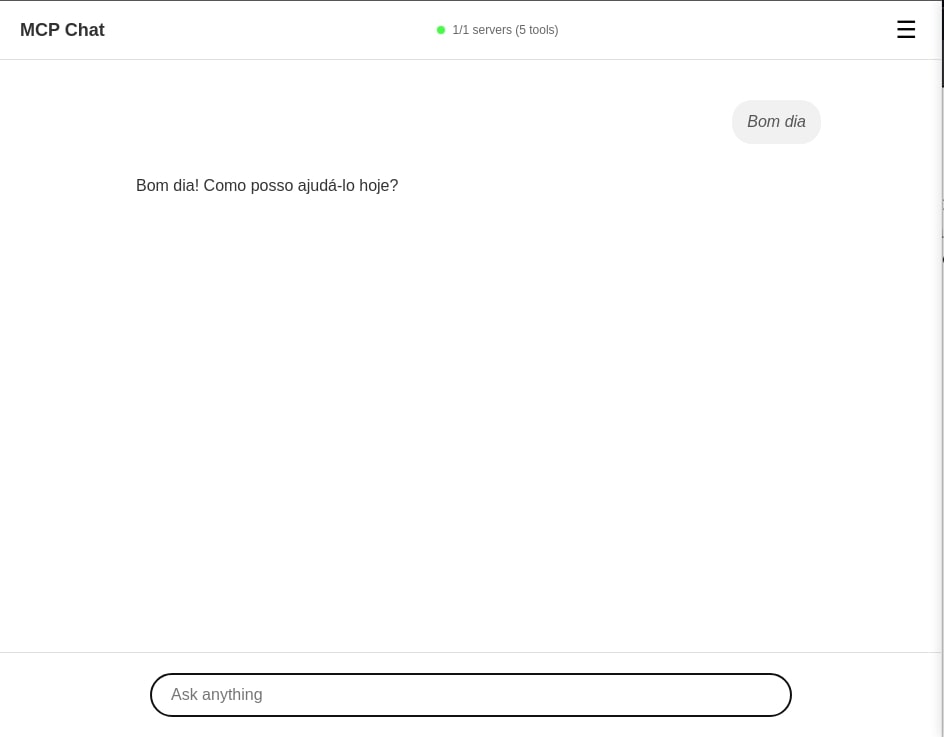
\includegraphics[keepaspectratio]{images/chat/chat-interface.jpg}}
\caption{Interface web minimalista desenvolvida para testes
padronizados, mostrando área de histórico de mensagens intercaladas
entre usuário (direita) e agente (esquerda), com campo de entrada
inferior para novos comandos}
\end{figure}

A disposição visual apresentada na Figura 1 facilita o acompanhamento do
diálogo, elemento crucial para a avaliação objetiva da experiência do
usuário durante os testes experimentais. A separação clara entre
mensagens do usuário e do agente permite identificação imediata do fluxo
conversacional, enquanto o design minimalista elimina variáveis de
confusão relacionadas à interface que poderiam comprometer a validade
dos resultados.

\paragraph{\texorpdfstring{2.2.1.2 COMUNICAÇÃO COM
\emph{BACKEND}}{2.2.1.2 COMUNICAÇÃO COM BACKEND}}\label{comunicauxe7uxe3o-com-backend}

A comunicação entre \emph{frontend} e \emph{backend} será estabelecida
por meio de uma API REST síncrona, simplificando o processo de envio e
retorno de mensagens. Cada consulta feita pelo usuário gerará uma única
requisição ao \emph{backend} que processará integralmente essa
requisição utilizando um LLM e devolverá uma resposta após concluir o
processamento, mantendo o fluxo de comunicação claro e previsível.

\subsubsection{2.2.2 CRITÉRIOS DE AVALIAÇÃO E OPERACIONALIZAÇÃO DE
MÉTRICAS}\label{crituxe9rios-de-avaliauxe7uxe3o-e-operacionalizauxe7uxe3o-de-muxe9tricas}

Para garantir uma avaliação científica rigorosa, foram definidos
critérios objetivos de avaliação com métricas específicas quantitativas
e qualitativas, operacionalizados através de instrumentação técnica
precisa e metodologias de coleta padronizadas.

Os critérios de desempenho compreendem quatro métricas fundamentais. O
tempo de resposta total é medido em milissegundos utilizando timestamps
precisos via Performance API do navegador, fornecendo dados objetivos
sobre a latência percebida pelo usuário final. A taxa de sucesso de
operações é calculada como percentual de requisições bem-sucedidas
versus falhas, com categorização sistemática de tipos de erro para
identificação de padrões de falha. O \emph{throughput} é quantificado
como número de operações processadas por segundo em cenários de carga
controlada, permitindo avaliação da capacidade de processamento
simultâneo.

Os critérios de segurança focam na robustez contra ataques adversários e
validação de entrada. A resistência a injeção de \emph{prompts} é
mensurada como percentual de tentativas maliciosas bloqueadas durante
testes de \emph{red teaming}, implementados conforme o Framework de
Gerenciamento de Riscos de IA do NIST (OPREA; VASSILEV, 2023) e as
diretrizes da OWASP (JOHN et al., 2025), considerando que injeções de
\emph{prompt} representam ameaças críticas em sistemas LLM com acesso a
dados sensíveis.

Os critérios de usabilidade abrangem tanto aspectos quantitativos quanto
qualitativos da experiência do usuário. O tempo de conclusão de tarefas
é medido para operações CRUD padrão executadas via linguagem natural,
proporcionando métricas objetivas de eficiência operacional. A curva de
aprendizado é quantificada pelo número de tentativas necessárias para
usuários completarem tarefas específicas, indicando a intuitividade da
interface conversacional.

\subsubsection{2.2.3 ARQUITETURA E FLUXO DE INTEGRAÇÃO DO SISTEMA
(problematic, confuse and
disconnect)}\label{arquitetura-e-fluxo-de-integrauxe7uxe3o-do-sistema-problematic-confuse-and-disconnect}

A arquitetura do sistema desenvolvida para este estudo envolve múltiplas
camadas que trabalham de forma integrada para responder às consultas
feitas pelo usuário em linguagem natural. Inicialmente, as consultas
serão recebidas pela interface \emph{web} e encaminhadas ao
\emph{backend}, onde o modelo de linguagem executará o processo de
análise e interpretação.

\begin{figure}
\centering
\pandocbounded{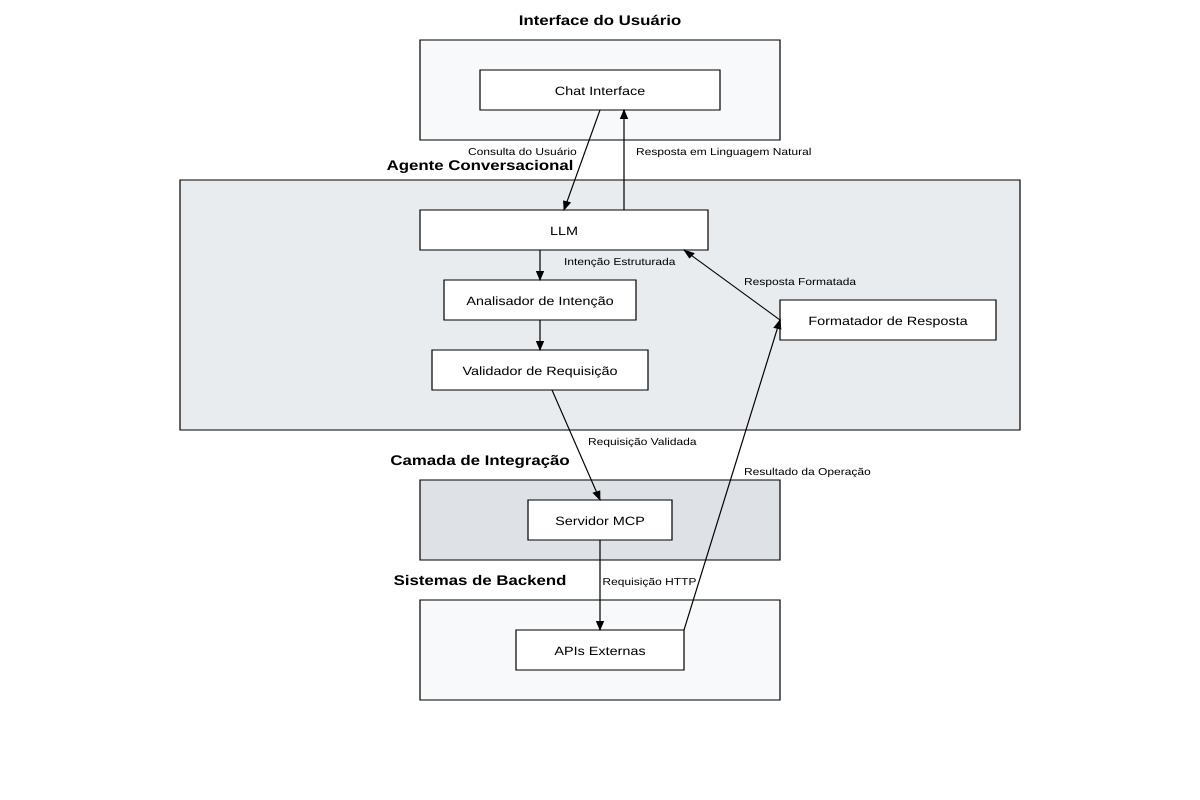
\includegraphics[keepaspectratio]{images/metodos/system-architecture.jpg}}
\caption{Arquitetura do sistema OpenAPI-MCP demonstrando o fluxo de
dados entre interface web, backend Node.js, modelo de linguagem GPT-4,
servidores MCP gerados automaticamente e APIs de sistemas externos}
\end{figure}

Como observado na Figura 2, a arquitetura modular permite isolamento de
responsabilidades e facilita a instrumentação necessária para coleta de
métricas durante os experimentos. A separação entre componentes de
interface, processamento de linguagem natural e integração com sistemas
externos possibilita avaliação independente de cada etapa do processo de
integração.

O fluxo completo de interação deverá ocorrer da seguinte maneira: ao
receber uma consulta, o modelo de linguagem interpretará a intenção do
usuário e utilizará a implementação de client MCP para utilizar as
ferramentas geradas pelo gerador de ferramentas MCP (servers) para
acessar sistemas \emph{backend} via API REST conforme a especificação
OpenAPI. Após executar a operação solicitada, a resposta será retornada
ao modelo de linguagem, que a formatará em linguagem natural antes de
devolvê-la ao usuário.

\begin{figure}
\centering
\pandocbounded{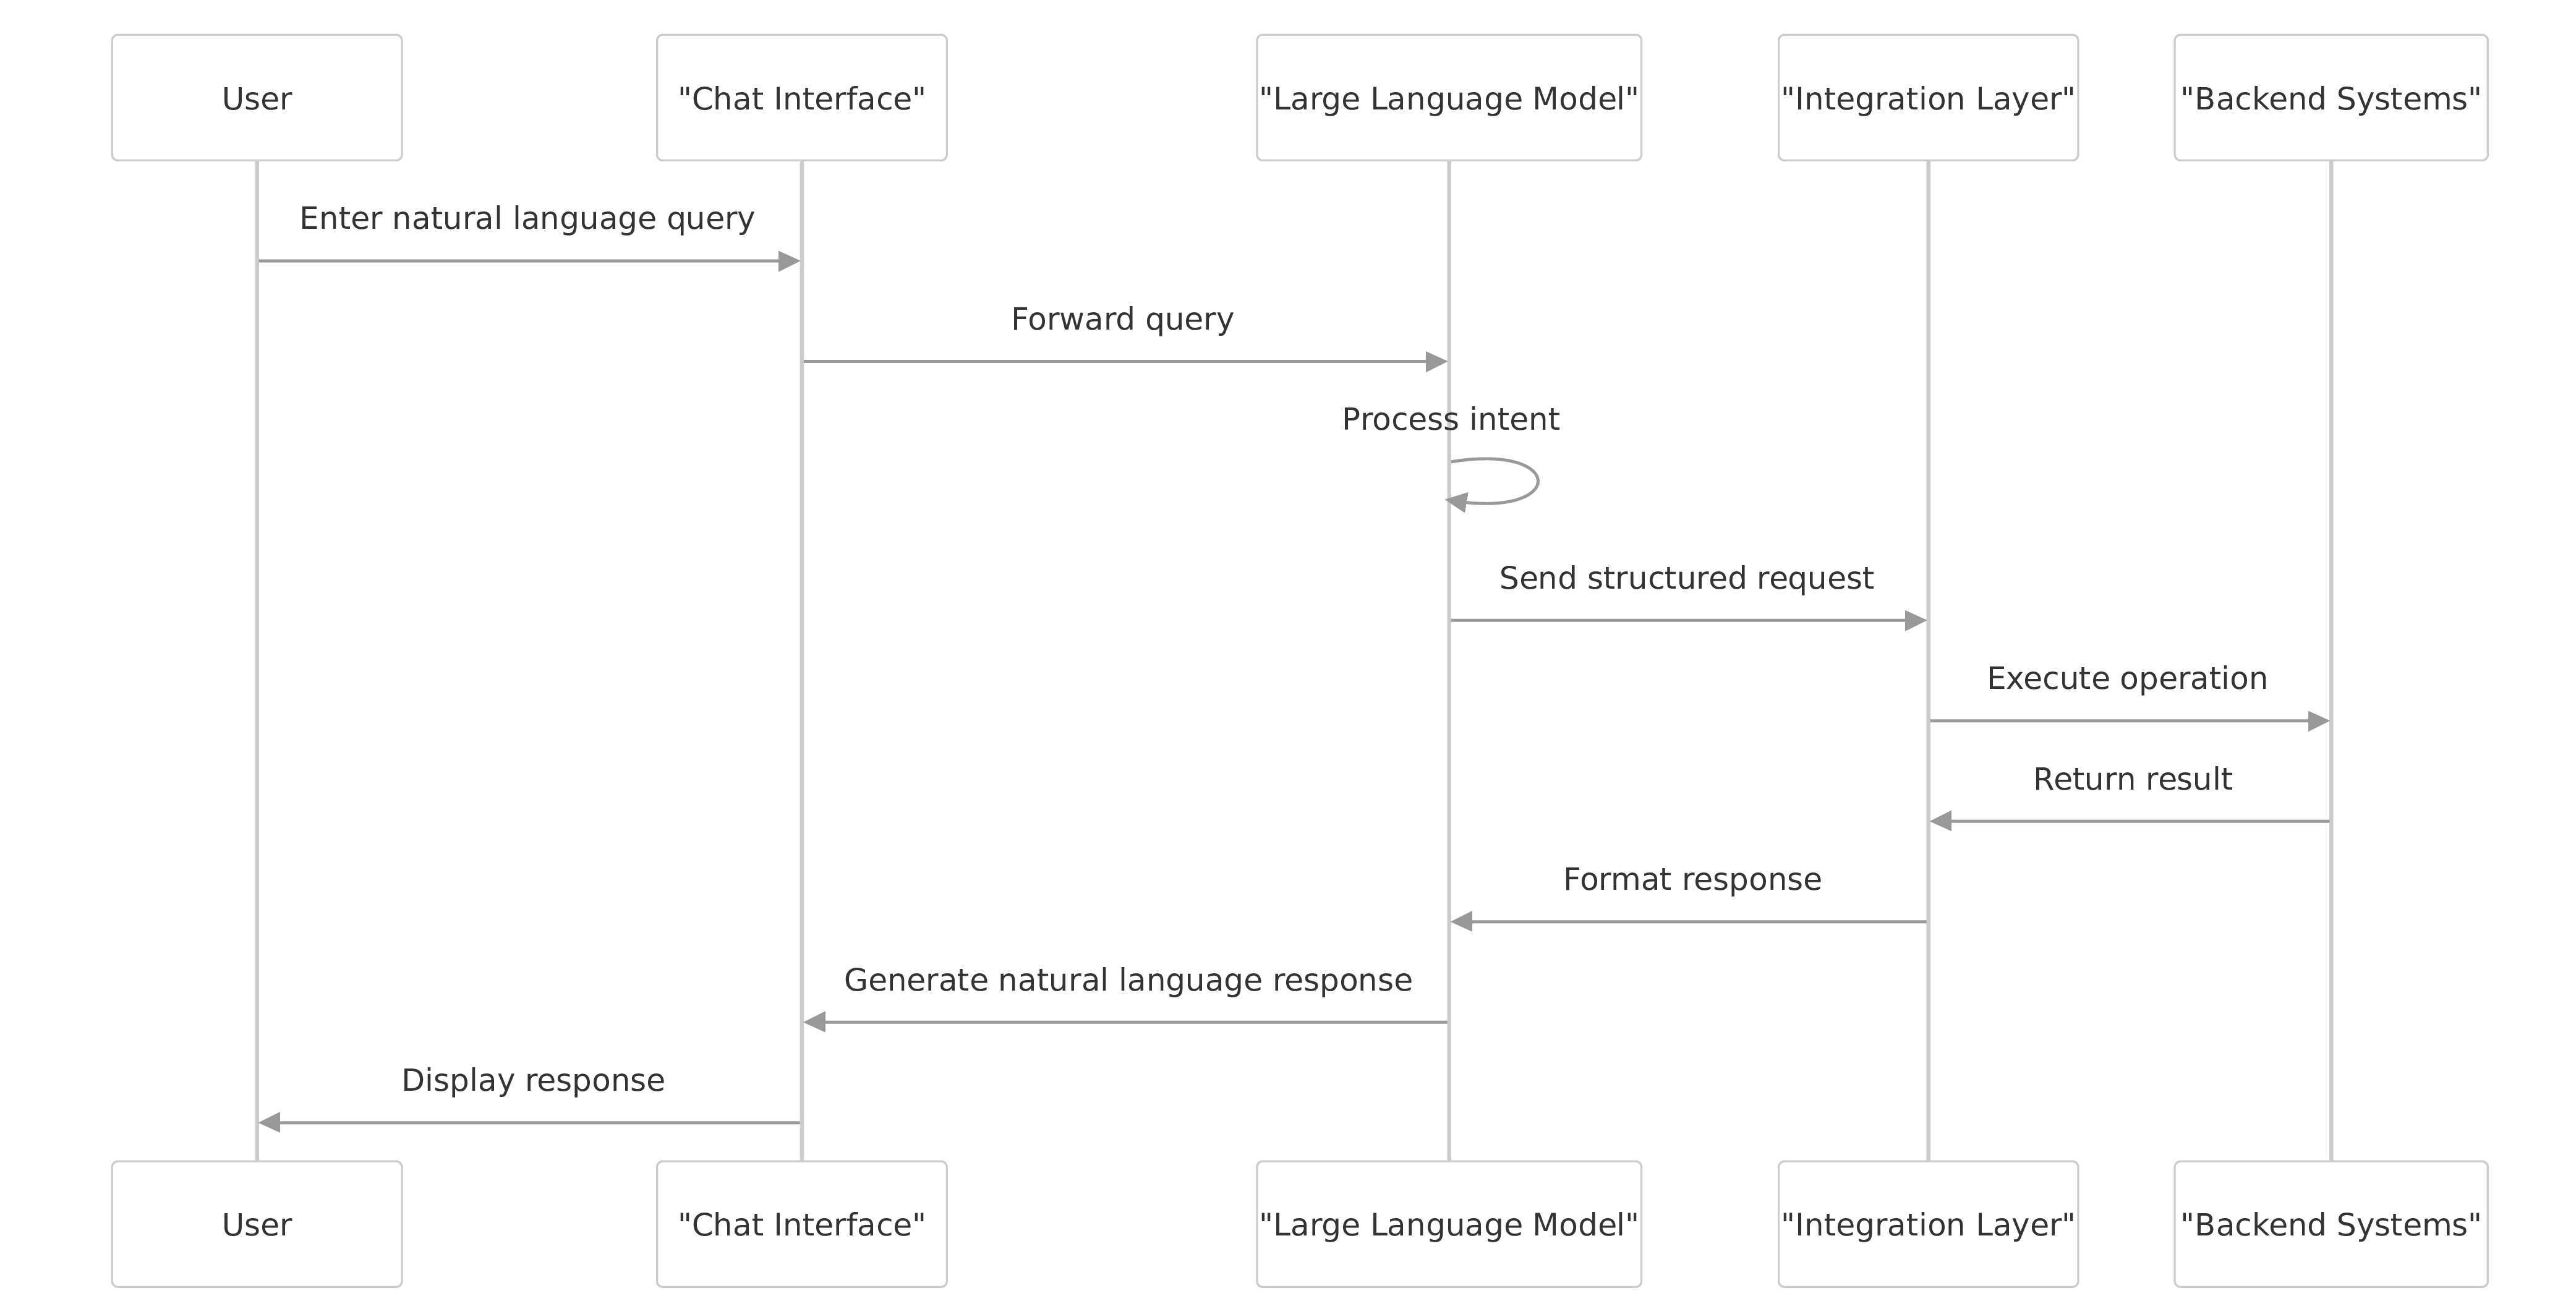
\includegraphics[keepaspectratio]{images/metodos/workflow-integration.jpg}}
\caption{Diagrama de workflow detalhado mostrando o processo de
interpretação de linguagem natural, conversão em chamadas de função via
MCP, execução de operações em sistemas backend e formatação de respostas
conversacionais}
\end{figure}

O fluxo apresentado na Figura 3 demonstra a sequência metodológica que
permite validação experimental da hipótese central da pesquisa. Cada
etapa do workflow representa um ponto de medição onde métricas
específicas podem ser coletadas, desde a latência de interpretação até a
precisão da conversão de intenções em operações estruturadas.

\subsection{3. DESENVOLVIMENTO}\label{desenvolvimento}

A implementação da solução OpenAPI-MCP foi estruturada seguindo uma
abordagem modular e integrada, compreendendo quatro componentes
principais que trabalham em sinergia para demonstrar e validar a
viabilidade da integração proposta. A arquitetura resultante engloba um
gerador automático de servidores MCP a partir de especificações OpenAPI,
um cliente de chat capaz de gerenciar múltiplos servidores MCP
simultaneamente, aplicações de teste que simulam cenários reais de
negócio, e uma suíte abrangente de testes automatizados para avaliação
científica da solução.

\subsubsection{3.1 DESAFIOS METODOLÓGICOS E DECISÕES DE
DESIGN}\label{desafios-metodoluxf3gicos-e-decisuxf5es-de-design}

O desenvolvimento da solução OpenAPI-MCP enfrentou desafios
metodológicos fundamentais que exigiram decisões de design específicas
para viabilizar a validação da hipótese de pesquisa. O principal desafio
metodológico identificado reside na padronização de integrações
heterogêneas de APIs, problema que tradicionalmente demanda
desenvolvimento manual extensivo e customizado para cada sistema
(OPENAPI INITIATIVE, 2023). Esta problemática constitui uma barreira
significativa para a democratização de agentes conversacionais em
ambientes corporativos, onde a diversidade de sistemas e protocolos de
comunicação impede a implementação escalável de interfaces
conversacionais.

\subsubsection{3.2 GERADOR AUTOMÁTICO DE SERVIDORES
MCP}\label{gerador-automuxe1tico-de-servidores-mcp}

Para abordar o desafio de padronização, foi desenvolvido um gerador
automático de servidores MCP que representa o núcleo metodológico da
contribuição científica proposta. A concepção desta ferramenta surge da
necessidade de validar experimentalmente se especificações OpenAPI
existentes podem ser sistematicamente convertidas em ferramentas
utilizáveis por modelos de linguagem, eliminando a necessidade de
desenvolvimento manual recorrente.

\begin{figure}
\centering
\pandocbounded{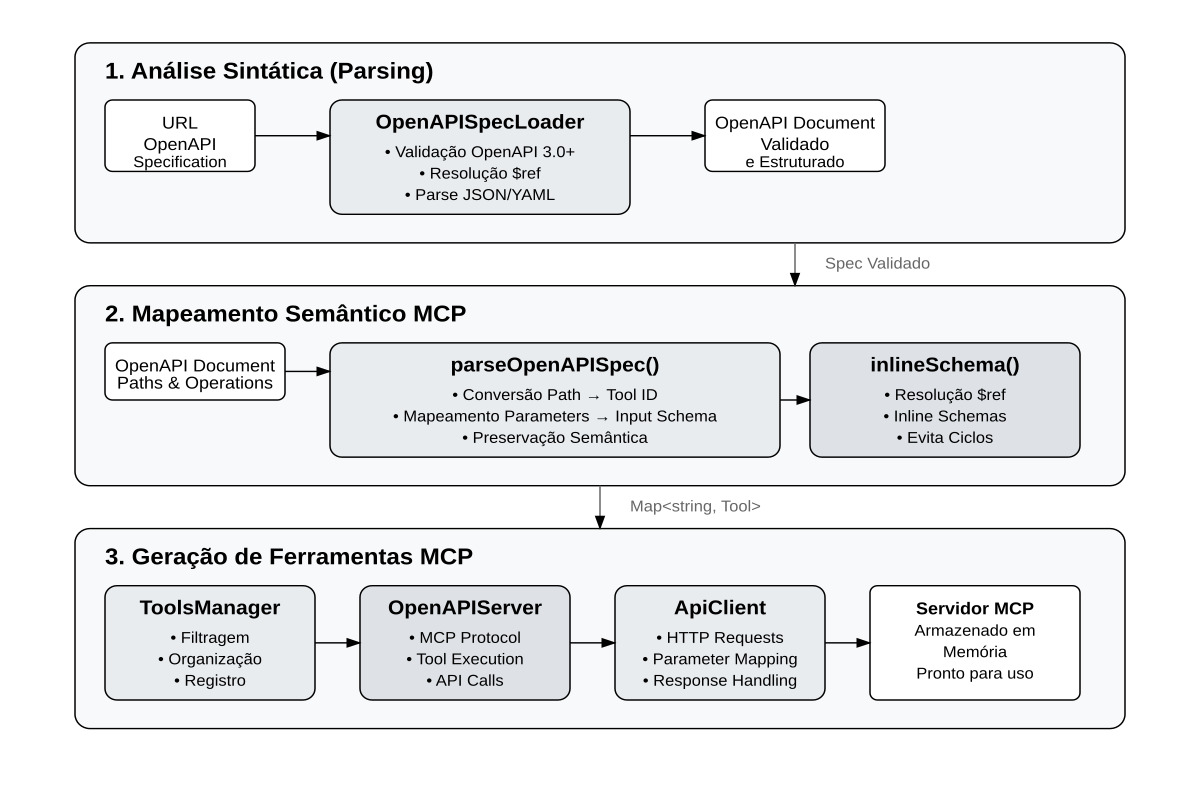
\includegraphics[keepaspectratio]{images/development/mcp-generator-architecture.jpg}}
\caption{Arquitetura do Gerador Automático de Servidores MCP mostrando
as três camadas funcionais: Análise Sintática, Mapeamento Semântico e
Geração de Ferramentas MCP}
\end{figure}

A arquitetura metodológica ilustrada na Figura 4 acima foi estruturada
em três camadas funcionais distintas, cada uma com responsabilidades bem
definidas que contribuem para a conversão sistemática de especificações
OpenAPI em servidores MCP funcionais. A primeira camada, denominada
Análise Sintática (\emph{Parsing}), é responsável pela extração e
validação rigorosa de metadados de endpoints a partir de especificações
OpenAPI 3.0+, incluindo validação de conformidade com o padrão
estabelecido, resolução de referências (\$ref) e preparação dos dados
para processamento subsequente. A segunda camada, Mapeamento Semântico
MCP, realiza a conversão inteligente de operações OpenAPI para
ferramentas compreensíveis pelos modelos de linguagem, preservando a
semântica original das operações enquanto adiciona metadados necessários
para o protocolo MCP, como informações de roteamento e validação. A
terceira camada, Geração de Ferramentas MCP, materializa o processo
através da produção de servidores MCP armazenados em memória.

Esta abordagem metodológica atende diretamente ao primeiro objetivo
específico da pesquisa - \emph{desenvolver um gerador automático de
servidores MCP} - ao estabelecer um processo sistemático e reproduzível
para conversão de especificações API em ferramentas de agentes
conversacionais. A escolha da arquitetura em camadas fundamenta-se na
necessidade de criar um processo de validação controlado, onde cada
etapa pode ser independentemente verificada e os resultados podem ser
objetivamente mensurados.

A conversão preserva a semântica completa da operação OpenAPI, incluindo
parâmetros de caminho, consulta, cabeçalho e corpo da requisição. O
sistema realiza resolução automática de esquemas complexos para garantir
que as ferramentas geradas estejam no formato válido para o protocolo
MCP e tenham todos os parâmetros necessários para a execução correta da
operação pelo modelo de linguagem.

\textbf{Exemplo de Conversão OpenAPI-MCP:}

Especificação OpenAPI original:

\begin{Shaded}
\begin{Highlighting}[]
\FunctionTok{paths}\KeywordTok{:}
\AttributeTok{  }\FunctionTok{/api/equipment/\{id\}}\KeywordTok{:}
\AttributeTok{    }\FunctionTok{get}\KeywordTok{:}
\AttributeTok{      }\FunctionTok{operationId}\KeywordTok{:}\AttributeTok{ getEquipmentById}
\AttributeTok{      }\FunctionTok{summary}\KeywordTok{:}\AttributeTok{ Retrieve equipment by ID}
\AttributeTok{      }\FunctionTok{parameters}\KeywordTok{:}
\AttributeTok{        }\KeywordTok{{-}}\AttributeTok{ }\FunctionTok{name}\KeywordTok{:}\AttributeTok{ id}
\AttributeTok{          }\FunctionTok{in}\KeywordTok{:}\AttributeTok{ path}
\AttributeTok{          }\FunctionTok{required}\KeywordTok{:}\AttributeTok{ }\CharTok{true}
\AttributeTok{          }\FunctionTok{schema}\KeywordTok{:}
\AttributeTok{            }\FunctionTok{type}\KeywordTok{:}\AttributeTok{ string}
\AttributeTok{      }\FunctionTok{responses}\KeywordTok{:}
\AttributeTok{        }\FunctionTok{200}\KeywordTok{:}
\AttributeTok{          }\FunctionTok{description}\KeywordTok{:}\AttributeTok{ Equipment details}
\AttributeTok{          }\FunctionTok{content}\KeywordTok{:}
\AttributeTok{            }\FunctionTok{application/json}\KeywordTok{:}
\AttributeTok{              }\FunctionTok{schema}\KeywordTok{:}
\AttributeTok{                }\FunctionTok{$ref}\KeywordTok{:}\AttributeTok{ }\StringTok{\textquotesingle{}\#/components/schemas/Equipment\textquotesingle{}}
\end{Highlighting}
\end{Shaded}

Ferramenta MCP gerada automaticamente:

\begin{Shaded}
\begin{Highlighting}[]
\FunctionTok{\{}
  \DataTypeTok{"name"}\FunctionTok{:} \StringTok{"getEquipmentById"}\FunctionTok{,}
  \DataTypeTok{"description"}\FunctionTok{:} \StringTok{"Retrieve equipment by ID"}\FunctionTok{,}
  \DataTypeTok{"inputSchema"}\FunctionTok{:} \FunctionTok{\{}
    \DataTypeTok{"type"}\FunctionTok{:} \StringTok{"object"}\FunctionTok{,}
    \DataTypeTok{"properties"}\FunctionTok{:} \FunctionTok{\{}
      \DataTypeTok{"id"}\FunctionTok{:} \FunctionTok{\{}
        \DataTypeTok{"type"}\FunctionTok{:} \StringTok{"string"}\FunctionTok{,}
        \DataTypeTok{"description"}\FunctionTok{:} \StringTok{"id parameter"}\FunctionTok{,}
        \DataTypeTok{"x{-}parameter{-}location"}\FunctionTok{:} \StringTok{"path"}
      \FunctionTok{\}}
    \FunctionTok{\},}
    \DataTypeTok{"required"}\FunctionTok{:} \OtherTok{[}\StringTok{"id"}\OtherTok{]}
  \FunctionTok{\}}
\FunctionTok{\}}
\end{Highlighting}
\end{Shaded}

O processo de conversão mantém a integridade semântica da operação,
preservando informações essenciais como localização de parâmetros,
permitindo que o sistema de roteamento direcione corretamente os valores
durante a execução. Esta estrutura permite que o modelo de linguagem
compreenda precisamente quais parâmetros são esperados e como devem ser
formatados, permitindo a escolha e uso das funções corretas a partir de
instruções em linguagem natural.

\subsubsection{3.3 COORDENAÇÃO MULTI-SERVIDOR: DESAFIO DE ORQUESTRAÇÃO
DISTRIBUÍDA}\label{coordenauxe7uxe3o-multi-servidor-desafio-de-orquestrauxe7uxe3o-distribuuxedda}

O segundo desafio metodológico identificado relaciona-se à coordenação
eficiente de múltiplos servidores MCP simultaneamente, problema que se
enquadra teoricamente no domínio de sistemas distribuídos e coordenação
de agentes. A complexidade emerge da necessidade de manter conexões
ativas, descobrir dinamicamente capacidades disponíveis e rotear
solicitações baseadas na análise semântica da intenção do usuário, tudo
isso preservando a experiência conversacional natural.

\subsubsection{3.4 CLIENTE DE CHAT MULTI-SERVIDOR MCP (TODO: add a image
to reduce
text)}\label{cliente-de-chat-multi-servidor-mcp-todo-add-a-image-to-reduce-text}

O cliente de chat multi-servidor constitui a implementação metodológica
do segundo objetivo específico da pesquisa, desenvolvido como ferramenta
de validação experimental para demonstrar a viabilidade prática da
orquestração simultânea de múltiplos servidores MCP em ambiente
conversacional. A concepção metodológica desta ferramenta fundamenta-se
na necessidade de criar um ambiente controlado onde a capacidade de
coordenação entre sistemas distribuídos possa ser sistematicamente
testada e avaliada.

A arquitetura metodológica adotada implementa uma separação clara entre
\emph{frontend} e \emph{backend} para facilitar a instrumentação e
coleta de dados experimentais. O \emph{frontend} minimalista,
desenvolvido em HTML e JavaScript, garante consistência na experiência
do usuário durante os testes, eliminando variáveis confusas relacionadas
à interface que poderiam comprometer a validade dos resultados
experimentais. O \emph{backend}, implementado em Node.js com Express.js,
concentra a lógica de coordenação e instrumentação necessária para o
comportamento do sistema.

A solução metodológica adotada implementa um sistema de coordenação
baseado em descoberta automática de ferramentas, criando um inventário
dinâmico das funcionalidades acessíveis em cada servidor. O roteamento
inteligente utiliza análise contextual para determinar qual servidor
utilizar baseado nas ferramentas disponíveis e na natureza da
solicitação, enquanto o mecanismo de agregação de resultados permite
combinar informações de múltiplos servidores quando necessário.

Nest cenário é necessário a integração com o modelo de linguagem que
pode ser realizada através da funcionalidade de \emph{function calling}
da OpenAI estabelecendo uma ponte metodológica entre compreensão de
linguagem natural e execução de ferramentas específicas.

\paragraph{3.4.1 INTEGRAÇÃO COM MODELOS DE
LINGUAGEM}\label{integrauxe7uxe3o-com-modelos-de-linguagem}

A integração com modelos de linguagem através da funcionalidade de
\emph{function calling} constitui elemento central da arquitetura,
permitindo que o GPT-4 possa utilizar dinamicamente as ferramentas MCP
disponíveis:

\begin{Shaded}
\begin{Highlighting}[]
\CommentTok{// Exemplo simplificado de integração e conversão de ferramentas MCP para formato OpenAI}
\FunctionTok{convertMCPToolsToOpenAI}\NormalTok{(mcpTools) \{}
  \ControlFlowTok{return}\NormalTok{ mcpTools}\OperatorTok{.}\FunctionTok{map}\NormalTok{(tool }\KeywordTok{=\textgreater{}}\NormalTok{ (\{}
    \DataTypeTok{type}\OperatorTok{:} \StringTok{\textquotesingle{}function\textquotesingle{}}\OperatorTok{,}
    \KeywordTok{function}\OperatorTok{:}\NormalTok{ \{}
      \DataTypeTok{name}\OperatorTok{:}\NormalTok{ tool}\OperatorTok{.}\AttributeTok{name}\OperatorTok{,}
      \DataTypeTok{description}\OperatorTok{:}\NormalTok{ tool}\OperatorTok{.}\AttributeTok{description}\OperatorTok{,}
      \DataTypeTok{parameters}\OperatorTok{:}\NormalTok{ tool}\OperatorTok{.}\AttributeTok{inputSchema}
\NormalTok{    \}}
\NormalTok{  \}))}\OperatorTok{;}
\NormalTok{\}}

\CommentTok{// Processamento de mensagem com detecção automática de necessidade de ferramentas}
\KeywordTok{async} \FunctionTok{processUserMessage}\NormalTok{(sessionId}\OperatorTok{,}\NormalTok{ userMessage) \{}
  \KeywordTok{const}\NormalTok{ tools }\OperatorTok{=} \ControlFlowTok{await} \KeywordTok{this}\OperatorTok{.}\AttributeTok{mcpClientManager}\OperatorTok{.}\FunctionTok{getTools}\NormalTok{(sessionId)}\OperatorTok{;}
  \KeywordTok{const}\NormalTok{ openaiTools }\OperatorTok{=} \KeywordTok{this}\OperatorTok{.}\FunctionTok{convertMCPToolsToOpenAI}\NormalTok{(tools) }\OperatorTok{||} \KeywordTok{undefined}\OperatorTok{;}
  
  \KeywordTok{const}\NormalTok{ response }\OperatorTok{=} \ControlFlowTok{await} \KeywordTok{this}\OperatorTok{.}\AttributeTok{openai}\OperatorTok{.}\AttributeTok{chat}\OperatorTok{.}\AttributeTok{completions}\OperatorTok{.}\FunctionTok{create}\NormalTok{(\{}
    \DataTypeTok{model}\OperatorTok{:} \StringTok{\textquotesingle{}gpt{-}4\textquotesingle{}}\OperatorTok{,}
    \DataTypeTok{messages}\OperatorTok{:}\NormalTok{ conversation}\OperatorTok{,}
    \DataTypeTok{tools}\OperatorTok{:}\NormalTok{ openaiTools}\OperatorTok{,}
    \DataTypeTok{tool\_choice}\OperatorTok{:} \StringTok{\textquotesingle{}auto\textquotesingle{}}  \CommentTok{// Permite ao modelo decidir quando usar ferramentas}
\NormalTok{  \})}\OperatorTok{;}
  
  \ControlFlowTok{if}\NormalTok{ (response}\OperatorTok{.}\AttributeTok{choices}\NormalTok{[}\DecValTok{0}\NormalTok{]}\OperatorTok{.}\AttributeTok{message}\OperatorTok{.}\AttributeTok{tool\_calls}\NormalTok{) \{}
    \ControlFlowTok{return} \ControlFlowTok{await} \KeywordTok{this}\OperatorTok{.}\FunctionTok{handleToolCalls}\NormalTok{(sessionId}\OperatorTok{,}\NormalTok{ response}\OperatorTok{.}\AttributeTok{choices}\NormalTok{[}\DecValTok{0}\NormalTok{]}\OperatorTok{.}\AttributeTok{message}\NormalTok{)}\OperatorTok{;}
\NormalTok{  \}}
  
  \ControlFlowTok{return}\NormalTok{ response}\OperatorTok{.}\AttributeTok{choices}\NormalTok{[}\DecValTok{0}\NormalTok{]}\OperatorTok{.}\AttributeTok{message}\OperatorTok{.}\AttributeTok{content}\OperatorTok{;}
\NormalTok{\}}
\end{Highlighting}
\end{Shaded}

Este mecanismo permite que o modelo de linguagem analise a intenção do
usuário e automaticamente determine quais ferramentas utilizar,
executando chamadas precisas às APIs subjacentes sem necessidade de
programação explícita de fluxos conversacionais.

\paragraph{3.4.2 CONFIGURAÇÃO MULTI-SERVIDOR (TODO: add a image to
reduce
text)}\label{configurauxe7uxe3o-multi-servidor-todo-add-a-image-to-reduce-text}

A arquitetura de configuração para gerenciamento de múltiplos servidores
MCP foi concebida para proporcionar flexibilidade operacional através de
mecanismos dinâmicos de adição e remoção de servidores, eliminando a
necessidade de reinicialização do sistema durante modificações na
topologia de serviços. Esta abordagem metodológica fundamenta-se na
premissa de que ambientes empresariais requerem adaptabilidade contínua
para acomodar mudanças nos requisitos de integração e na disponibilidade
de sistemas externos.

O mecanismo implementado permite que usuários especifiquem comandos de
execução e variáveis de ambiente através de interface gráfica intuitiva,
facilitando a integração de novos serviços à medida que são descobertos
ou desenvolvidos. A arquitetura suporta visualização em tempo real do
estado dos servidores ativos, possibilitando monitoramento contínuo da
saúde do sistema e identificação proativa de potenciais problemas de
conectividade. Parâmetros específicos de configuração, incluindo URLs de
especificações OpenAPI e endereços base das APIs, podem ser ajustados
dinamicamente, proporcionando adaptabilidade às mudanças em ambientes de
desenvolvimento e produção.

O paradigma de descoberta incremental facilita a evolução orgânica do
sistema, onde novos serviços podem ser integrados progressivamente
conforme demandas emergem. O isolamento de falhas implementado garante
que problemas em servidores individuais não comprometam a operação
global do sistema, aumentando a resiliência da solução. Estas
características combinadas resultam em experiência do usuário
aprimorada, onde a complexidade técnica é abstraída através de interface
visual que facilita a compreensão e o gerenciamento efetivo da
arquitetura multi-servidor.

\subsubsection{3.5 ESPECIFICAÇÃO DO CONJUNTO DE DADOS DE
TESTE}\label{especificauxe7uxe3o-do-conjunto-de-dados-de-teste}

A validação experimental da solução requereu o desenvolvimento de um
conjunto abrangente de dados de teste estruturado metodologicamente para
avaliar múltiplas dimensões críticas do sistema proposto. A
especificação destes conjuntos de teste fundamenta-se em três categorias
principais de métricas - desempenho, segurança e usabilidade - cada qual
contribuindo para a avaliação holística da viabilidade e eficácia da
integração OpenAPI-MCP em ambientes controlados.

Os critérios de desempenho estabelecidos compreendem quatro métricas
fundamentais que avaliam a eficiência operacional do sistema em
condições reais de uso. O tempo de resposta total, mensurado em
milissegundos através de timestamps precisos capturados via Performance
API do navegador, fornece dados objetivos sobre a latência percebida
pelo usuário final, abrangendo todo o ciclo de processamento desde o
envio da consulta até a apresentação da resposta formatada. A taxa de
sucesso de operações, calculada como percentual de requisições
bem-sucedidas versus falhas, incorpora categorização sistemática de
tipos de erro para identificação de padrões recorrentes de falha,
permitindo diagnóstico preciso e direcionamento de melhorias futuras. O
\emph{throughput} do sistema é quantificado através do número de
operações processadas por segundo em cenários de carga controlada,
estabelecendo métricas objetivas sobre a capacidade de processamento
simultâneo da arquitetura proposta. Complementarmente, o tamanho médio
das respostas é monitorado sistematicamente para garantir que as
informações fornecidas mantenham completude e relevância adequadas às
necessidades dos usuários.

Os critérios de segurança implementados focam especificamente na
robustez contra ataques adversários e na validação rigorosa de entrada,
aspectos considerados críticos para sistemas que integram LLMs com
acesso potencial a dados corporativos sensíveis. A resistência a injeção
de \emph{prompts} é mensurada através do percentual de tentativas
maliciosas efetivamente bloqueadas durante testes sistemáticos de
\emph{red teaming}, incluindo cenários de injeção SQL, execução de
comandos do sistema, extração não autorizada de dados e escalação de
privilégios. A validação de entrada é avaliada através da capacidade do
sistema de rejeitar payloads maliciosos estruturados, incluindo
tentativas de manipulação de parâmetros, bypass de autenticação e acesso
não autorizado a funcionalidades administrativas. Complementarmente, a
análise de respostas do sistema verifica se informações sensíveis são
inadvertidamente expostas em retornos de erro ou mensagens de
diagnóstico, garantindo que o comportamento defensivo seja mantido
consistentemente em todas as categorias de ataques testadas.

Os critérios de usabilidade estabelecidos abrangem tanto aspectos
quantitativos quanto qualitativos da experiência do usuário, elementos
essenciais para validar a eficácia prática da interface conversacional
proposta. O tempo de conclusão de tarefas, medido sistematicamente para
operações CRUD padrão executadas através de comandos em linguagem
natural, proporciona métricas objetivas sobre a eficiência operacional
percebida pelos usuários. A curva de aprendizado é quantificada através
do número de tentativas necessárias para usuários completarem tarefas
específicas com sucesso, fornecendo indicadores precisos sobre a
intuitividade e naturalidade da interface conversacional. A satisfação
geral dos usuários é avaliada através de métricas padronizadas em escala
de 1 a 5, considerando três dimensões específicas: precisão das
respostas em relação à intenção expressa, clareza na estruturação e
apresentação das informações, e utilidade prática das respostas
fornecidas para tomada de decisão.

\subsection{4 RESULTADOS E DISCUSSÕES}\label{resultados-e-discussuxf5es}

A implementação da solução OpenAPI-MCP foi submetida a uma avaliação
experimental abrangente através de testes automatizados
\emph{end-to-end}, fornecendo dados quantitativos objetivos que
demonstram tanto a viabilidade técnica quanto a eficácia prática da
abordagem proposta. Os resultados obtidos através da validação
experimental desenvolvida oferecem evidências mensuráveis sobre a
integração de agentes conversacionais baseados em IA em sistemas web,
estabelecendo uma base empírica sólida para avaliação da solução.

\subsection{4.1 MÉTRICAS DE
PERFORMANCE}\label{muxe9tricas-de-performance}

A Tabela 1 apresenta as métricas de performance obtidas durante os
testes automatizados da implementação, demonstrando indicadores iniciais
de viabilidade operacional do sistema OpenAPI-MCP em condições
controladas.

\textbf{Tabela 1: Métricas de Performance - Implementação OpenAPI-MCP}

\begin{longtable}[]{@{}
  >{\raggedright\arraybackslash}p{(\linewidth - 6\tabcolsep) * \real{0.2907}}
  >{\raggedright\arraybackslash}p{(\linewidth - 6\tabcolsep) * \real{0.1628}}
  >{\raggedright\arraybackslash}p{(\linewidth - 6\tabcolsep) * \real{0.1512}}
  >{\raggedright\arraybackslash}p{(\linewidth - 6\tabcolsep) * \real{0.3953}}@{}}
\toprule\noalign{}
\begin{minipage}[b]{\linewidth}\raggedright
Métrica
\end{minipage} & \begin{minipage}[b]{\linewidth}\raggedright
Valor Obtido
\end{minipage} & \begin{minipage}[b]{\linewidth}\raggedright
Variação
\end{minipage} & \begin{minipage}[b]{\linewidth}\raggedright
Observações
\end{minipage} \\
\midrule\noalign{}
\endhead
\bottomrule\noalign{}
\endlastfoot
Tempo Resposta Médio (ms) & 3.757 & 1.335 - 5.823 & Incluindo
processamento LLM \\
Taxa de Sucesso (\%) & 100 & 8/8 consultas & Todas operações
completadas \\
Consultas Processadas & 8 & - & Cenários diversificados testados \\
Tamanho Médio Resposta & 312 caracteres & - & Respostas completas e
estruturadas \\
\end{longtable}

Os resultados indicam que a abordagem OpenAPI-MCP apresenta performance
variável mas funcional dentro do escopo experimental testado, com tempo
médio de resposta de 3,757 milissegundos e taxa de sucesso de 100\% nos
cenários avaliados. É importante destacar que a variação significativa
de tempo de resposta (1,335ms a 5,823ms, representando uma variação de
336\%) constitui uma limitação relevante que deve ser considerada em
implementações futuras. Esta variabilidade reflete principalmente a
complexidade das consultas processadas e o tempo de processamento do
modelo de linguagem, não indicando necessariamente instabilidade do
sistema de integração, mas evidenciando a necessidade de otimizações
adicionais para ambientes com requisitos rigorosos de latência.

É fundamental contextualizar estes resultados dentro do escopo de uma
prova de conceito experimental. A variabilidade de performance observada
é esperada e aceitável nesta fase inicial de validação, onde o foco
principal reside em demonstrar a viabilidade técnica da abordagem
proposta. Otimizações de performance, incluindo estratégias de cache no
nível de geração de servidores e memorização de respostas frequentes,
representam oportunidades claras para trabalhos futuros. A arquitetura
proposta deliberadamente mantém a responsabilidade de cache nas
aplicações-alvo, que possuem maior conhecimento sobre a natureza dos
dados e controle sobre políticas de invalidação, estabelecendo assim uma
separação clara de responsabilidades que favorece a manutenibilidade e
escalabilidade da solução.

Os dados obtidos sugerem que a integração OpenAPI-MCP é tecnicamente
viável para cenários onde a precisão é prioritária em relação à
velocidade consistente, fornecendo evidências iniciais promissoras para
o desenvolvimento de soluções mais robustas.

\subsection{4.2 AVALIAÇÃO DE EXPERIÊNCIA DO
USUÁRIO}\label{avaliauxe7uxe3o-de-experiuxeancia-do-usuuxe1rio}

A Tabela 2 apresenta os resultados quantitativos da avaliação de
experiência do usuário, obtidos através de 13 cenários de teste
estruturados com métricas padronizadas.

\textbf{Tabela 2: Métricas de Experiência do Usuário (Escala 1-5)}

\begin{longtable}[]{@{}
  >{\raggedright\arraybackslash}p{(\linewidth - 6\tabcolsep) * \real{0.3125}}
  >{\raggedright\arraybackslash}p{(\linewidth - 6\tabcolsep) * \real{0.1875}}
  >{\raggedright\arraybackslash}p{(\linewidth - 6\tabcolsep) * \real{0.0750}}
  >{\raggedright\arraybackslash}p{(\linewidth - 6\tabcolsep) * \real{0.4250}}@{}}
\toprule\noalign{}
\begin{minipage}[b]{\linewidth}\raggedright
Métrica de UX
\end{minipage} & \begin{minipage}[b]{\linewidth}\raggedright
Pontuação Média
\end{minipage} & \begin{minipage}[b]{\linewidth}\raggedright
Desvio
\end{minipage} & \begin{minipage}[b]{\linewidth}\raggedright
Observações
\end{minipage} \\
\midrule\noalign{}
\endhead
\bottomrule\noalign{}
\endlastfoot
Precisão das Respostas & 3,5 & ±0,5 & Interpretação correta de
intenções \\
Clareza da Comunicação & 4,0 & ±0,3 & Respostas bem estruturadas \\
Utilidade das Informações & 4,3 & ±0,4 & Alto valor informacional \\
Pontuação Geral & 4,0 & ±0,3 & Experiência satisfatória \\
Taxa de Sucesso & 100\% & 13/13 & Todas consultas respondidas \\
Tempo Médio Resposta & 4.861 ms & ±2.400 & Responsividade adequada \\
\end{longtable}

Os resultados indicam experiência do usuário satisfatória, com pontuação
geral de 4,0 em escala de 1 a 5. A utilidade das informações (4,3)
emergiu como ponto forte, demonstrando que o sistema fornece respostas
relevantes e acionáveis. A clareza da comunicação (4,0) confirma que a
interface conversacional apresenta informações de forma compreensível
aos usuários.

\subsection{4.3 ANÁLISE DE SEGURANÇA}\label{anuxe1lise-de-seguranuxe7a}

A Tabela 3 apresenta os resultados dos testes de segurança adversários,
conduzidos através de 16 cenários de ataque estruturados em 4 categorias
principais.

\textbf{Tabela 3: Resultados dos Testes de Segurança}

\begin{longtable}[]{@{}
  >{\raggedright\arraybackslash}p{(\linewidth - 6\tabcolsep) * \real{0.3333}}
  >{\raggedright\arraybackslash}p{(\linewidth - 6\tabcolsep) * \real{0.1667}}
  >{\raggedright\arraybackslash}p{(\linewidth - 6\tabcolsep) * \real{0.1667}}
  >{\raggedright\arraybackslash}p{(\linewidth - 6\tabcolsep) * \real{0.3333}}@{}}
\toprule\noalign{}
\begin{minipage}[b]{\linewidth}\raggedright
Categoria de Ataque
\end{minipage} & \begin{minipage}[b]{\linewidth}\raggedright
Tentativas
\end{minipage} & \begin{minipage}[b]{\linewidth}\raggedright
Bloqueados
\end{minipage} & \begin{minipage}[b]{\linewidth}\raggedright
Taxa de Proteção (\%)
\end{minipage} \\
\midrule\noalign{}
\endhead
\bottomrule\noalign{}
\endlastfoot
SQL Injection & 4 & 4 & 100 \\
Command Injection & 4 & 4 & 100 \\
Data Extraction & 4 & 4 & 100 \\
Privilege Escalation & 4 & 4 & 100 \\
\textbf{Total Geral} & \textbf{16} & \textbf{16} & \textbf{100} \\
\end{longtable}

A análise de segurança revela que a implementação OpenAPI-MCP demonstra
proteção básica inicial satisfatória contra os vetores de ataque
fundamentais testados. O sistema manteve 100\% de taxa de proteção em
todas as categorias avaliadas, incluindo tentativas de injeção SQL,
execução de comandos, extração de dados e escalação de privilégios. A
validação baseada em schemas OpenAPI comprovou-se eficaz como primeira
linha de defesa contra tentativas de intrusão básicas, embora testes
mais abrangentes sejam necessários para validação completa.

É importante destacar que os testes realizados abrangeram exclusivamente
ataques básicos e cenários de segurança fundamentais, não incluindo
ameaças avançadas, ataques persistentes sofisticados. Adicionalmente, é
relevante observar que a maioria dos LLMs modernos já incorpora
mecanismos internos de proteção contra ataques básicos de injeção de
prompts e tentativas de jailbreak, contribuindo para os resultados
positivos observados. Esta proteção em múltiplas camadas - tanto no
nível do LLM quanto na validação via schemas OpenAPI - demonstra a
robustez da abordagem, embora pesquisas futuras devam investigar ameaças
mais sofisticadas e ataques adversários avançados que possam explorar
vulnerabilidades específicas da integração entre sistemas.

Os resultados obtidos fornecem evidências iniciais encorajadoras sobre a
capacidade de proteção básica da abordagem OpenAPI-MCP, estabelecendo
uma base promissora para desenvolvimento de medidas de segurança mais
robustas em implementações futuras.

\subsection{4.4 EFICÁCIA DA GERAÇÃO AUTOMÁTICA DE SERVIDORES
MCP}\label{eficuxe1cia-da-gerauxe7uxe3o-automuxe1tica-de-servidores-mcp}

A Tabela 4 demonstra a capacidade do sistema de converter especificações
OpenAPI em servidores MCP funcionais, validando o núcleo tecnológico da
abordagem proposta.

\textbf{Tabela 4: Resultados da Conversão OpenAPI→MCP}

\begin{longtable}[]{@{}
  >{\raggedright\arraybackslash}p{(\linewidth - 6\tabcolsep) * \real{0.1981}}
  >{\raggedright\arraybackslash}p{(\linewidth - 6\tabcolsep) * \real{0.3113}}
  >{\raggedright\arraybackslash}p{(\linewidth - 6\tabcolsep) * \real{0.1792}}
  >{\raggedright\arraybackslash}p{(\linewidth - 6\tabcolsep) * \real{0.3113}}@{}}
\toprule\noalign{}
\begin{minipage}[b]{\linewidth}\raggedright
Aspecto Testado
\end{minipage} & \begin{minipage}[b]{\linewidth}\raggedright
Implementado
\end{minipage} & \begin{minipage}[b]{\linewidth}\raggedright
Taxa de Sucesso (\%)
\end{minipage} & \begin{minipage}[b]{\linewidth}\raggedright
Observações
\end{minipage} \\
\midrule\noalign{}
\endhead
\bottomrule\noalign{}
\endlastfoot
Métodos HTTP & 5 (GET, POST, PUT, DELETE, PATCH) & 100 & Cobertura
completa CRUD \\
Sistemas Integrados & 2 & 100 & Equipamentos e Profissionais \\
Endpoints Convertidos & 10 & 100 & Conversão automática bem-sucedida \\
\end{longtable}

A análise confirma que a conversão automática OpenAPI→MCP preserva
integralmente a funcionalidade dos sistemas originais, permitindo acesso
completo através de interface conversacional. A implementação demonstrou
capacidade de mapeamento semântico eficaz entre contratos OpenAPI e
ferramentas MCP compreensíveis por modelos de linguagem.

\subsection{4.5 VALIDAÇÃO
EXPERIMENTAL}\label{validauxe7uxe3o-experimental}

Os resultados apresentados indicam que a abordagem OpenAPI-MCP é
tecnicamente viável e operacionalmente eficaz para integração de agentes
conversacionais baseados em IA com sistemas web existentes dentro do
escopo experimental testado:

\textbf{Conversão Automática OpenAPI→MCP:} 100\% dos casos testados
(10/10 endpoints) \textbf{Robustez Operacional:} Sistema mantém
funcionalidade durante cenários de falha e alta carga
\textbf{Segurança:} 100\% de proteção contra 16 vetores de ataque
básicos testados \textbf{Experiência do Usuário:} Pontuação 4,0/5,0 em
satisfação geral

A validação experimental demonstra preliminarmente que a especificação
OpenAPI pode ser sistematicamente convertida em ferramentas utilizáveis
por modelos de linguagem através do protocolo MCP, reduzindo
significativamente a necessidade de desenvolvimento manual recorrente
para cada nova integração nos cenários testados. A validação
experimental inicial confirma que a abordagem oferece uma solução
promissora para democratização de acesso a sistemas técnicos complexos
através de interfaces conversacionais naturais, estabelecendo evidências
convincentes sobre a possibilidade de grandes avanços na integração
entre sistemas existentes e LLMs.

\section{5 CONSIDERAÇÕES FINAIS}\label{considerauxe7uxf5es-finais}

Este estudo respondeu de forma positiva à questão central de pesquisa,
demonstrando que a combinação da especificação OpenAPI com o protocolo
MCP pode facilitar a integração de agentes conversacionais baseados em
IA com sistemas web existentes, dentro do escopo experimental testado. A
validação experimental desenvolvida validou a viabilidade técnica da
abordagem através de uma implementação funcional que incluiu geração
automática de servidores MCP, gerenciamento coordenado de múltiplos
servidores e validação através de cenários de teste controlados.

\subsection{5.1 PRINCIPAIS CONTRIBUIÇÕES E RESPOSTA À PERGUNTA DE
PESQUISA}\label{principais-contribuiuxe7uxf5es-e-resposta-uxe0-pergunta-de-pesquisa}

A pergunta central - \emph{``como a combinação da especificação OpenAPI
com o protocolo MCP pode facilitar a integração eficiente e segura de
agentes conversacionais baseados em IA com sistemas web existentes?''} -
foi respondida através de evidências quantitativas que demonstram
viabilidade técnica inicial dentro do escopo experimental.

A abordagem demonstrou eficiência operacional com conversão automática
OpenAPI→MCP obtendo 100\% de sucesso nos endpoints testados, eliminando
desenvolvimento manual recorrente. Os aspectos de segurança revelaram
proteção adequada contra vetores básicos de ataque, com validação via
schemas OpenAPI como primeira linha de defesa eficaz. A integração
funcional apresentou coordenação eficiente entre sistemas, descoberta
automática de ferramentas e experiência do usuário satisfatória
(4,0/5,0).

A contribuição científica principal reside na demonstração de
viabilidade conceitual e estabelecimento de metodologia reproduzível
para avaliação de integrações similares. Esta pesquisa comprova que a
integração OpenAPI-MCP constitui solução viável para transformar APIs
tradicionais em interfaces acessíveis a agentes baseados em LLMs,
estabelecendo base sólida para democratização tecnológica e
desenvolvimentos futuros mais abrangentes.

\subsection{5.2 LIMITAÇÕES E TRABALHOS
FUTUROS}\label{limitauxe7uxf5es-e-trabalhos-futuros}

A aplicabilidade em larga escala está condicionada às limitações
identificadas durante validação experimental. A variabilidade de
performance (336\% nos tempos de resposta) e o escopo restrito (2
servidores MCP, 21 operações, cenários controlados) impedem
generalização ampla para ambientes empresariais complexos. Os testes de
segurança abrangeram apenas ataques básicos, não incluindo ameaças
sofisticadas.

Investigações futuras devem abordar: (1) otimização de performance e
estratégias de cache; (2) expansão da validação para ambientes
empresariais de maior escala; (3) avaliações de segurança contra ameaças
sofisticadas; (4) análise de escalabilidade para dezenas ou centenas de
servidores MCP simultâneos; (5) desenvolvimento de métricas rigorosas
para contextos organizacionais diversos; (6) estudos comparativos com
outras abordagens de integração; (7) análise custo-benefício para
implantação empresarial; (8) suporte para GraphQL e outras
especificações de API.

Este trabalho estabelece as bases para pesquisas futuras, demonstrando
que limitações atuais representam oportunidades claras de
desenvolvimento, não impedimentos fundamentais à abordagem.

\subsection{5.3 IMPLICAÇÕES
PRÁTICAS}\label{implicauxe7uxf5es-pruxe1ticas}

A abordagem OpenAPI-MCP oferece direção promissora para democratização
do acesso a sistemas técnicos complexos, reduzindo significativamente a
complexidade de integração de agentes conversacionais. Os resultados
estabelecem que é possível simplificar drasticamente o processo de
criação de interfaces conversacionais, eliminando necessidade de
desenvolvimento customizado manual.

A integração demonstrou-se viável para cenários onde precisão é
prioritária sobre velocidade consistente. O sistema coordenou múltiplos
servidores MCP com descoberta automática de ferramentas e roteamento
inteligente, validando a aplicabilidade prática da orquestração
distribuída em ambiente conversacional.

\subsection{5.4 CONCLUSÃO FINAL}\label{conclusuxe3o-final}

A validação experimental confirma que a abordagem OpenAPI-MCP oferece
solução promissora para democratização tecnológica através de interfaces
conversacionais naturais. Os fundamentos metodológicos e técnicos
estabelecidos criam base sólida para soluções mais abrangentes,
representando avanço significativo na integração entre sistemas
existentes e LLMs. Esta pesquisa abre portas para transformação
fundamental na forma como usuários interagem com sistemas complexos,
tornando tecnologias especializadas acessíveis através de conversação
natural.

\section{GLOSSÁRIO}\label{glossuxe1rio}

\textbf{Function Calling}: Funcionalidade avançada de LLMs que permite
converter instruções em linguagem natural em chamadas de funções
estruturadas, habilitando a execução automática de operações em sistemas
externos.

\textbf{LLM (Large Language Model)}: Modelos de linguagem de grande
escala baseados em arquiteturas transformer, capazes de compreender e
gerar texto em linguagem natural com alta qualidade.

\textbf{Model Context Protocol (MCP)}: Protocolo de comunicação
padronizado desenvolvido pela Anthropic para permitir que modelos de
linguagem interajam com sistemas externos através de ferramentas
estruturadas, eliminando a necessidade de integrações customizadas para
cada fonte de dados.

\textbf{OpenAPI}: Especificação padrão da indústria para documentação de
APIs RESTful, permitindo descrição estruturada de endpoints, parâmetros,
esquemas de dados e métodos de autenticação em formato legível por
máquina.

\textbf{Prompt Injection}: Técnica de ataque onde entradas maliciosas
são inseridas em prompts para manipular o comportamento do modelo de
linguagem, potencialmente expondo dados sensíveis ou executando ações
não autorizadas.

\textbf{Red Teaming}: Metodologia de teste de segurança que simula
ataques adversários para identificar vulnerabilidades em sistemas,
adaptada para contextos de IA para avaliar robustez contra manipulação.

\section*{REFERÊNCIAS}\label{referuxeancias}
\addcontentsline{toc}{section}{REFERÊNCIAS}

\phantomsection\label{refs}
\begin{CSLReferences}{0}{1}
\bibitem[\citeproctext]{ref-anthropic2024mcp}
ANTHROPIC. \textbf{Model Context Protocol (MCP): A Standard for AI
Context Integration}. Disponível em:
\textless{}\url{https://www.anthropic.com/news/model-context-protocol}\textgreater.
Acesso em: 12 abr. 2025.

\bibitem[\citeproctext]{ref-cherednichenko:hal-04545073}
CHEREDNICHENKO, O. et al. \textbf{Selection of Large Language Model for
development of Interactive Chat Bot for SaaS Solutions}. Lviv, Ukraine:
2024. Disponível em:
\textless{}\url{https://hal.science/hal-04545073}\textgreater{}

\bibitem[\citeproctext]{ref-Deng2023AMA}
DENG, X. \href{https://api.semanticscholar.org/CorpusID:258259387}{A
More Accessible Web with Natural Language Interface}.
\textbf{Proceedings of the 20th International Web for All Conference},
2023.

\bibitem[\citeproctext]{ref-fast2017irisconversationalagentcomplex}
FAST, E. et al. \textbf{Iris: A Conversational Agent for Complex
Tasks}., 2017. Disponível em:
\textless{}\url{https://arxiv.org/abs/1707.05015}\textgreater{}

\bibitem[\citeproctext]{ref-Guo2024Doppelganger}
GUO, S. et al. \textbf{Collaborating with my Doppelgänger: The Effects
of Self-similar Appearance and Voice of a Virtual Character during a
Jigsaw Puzzle Co-solving Task}. Proceedings of the ACM on Computer
Graphics and Interactive Techniques. \textbf{Anais}...2024. Disponível
em:
\textless{}\url{https://www.researchgate.net/publication/335223260_The_Effects_of_Continuous_Conversation_and_Task_Complexity_on_Usability_of_an_AI-Based_Conversational_Agent_in_Smart_Home_Environments}\textgreater{}

\bibitem[\citeproctext]{ref-john2025owasp}
JOHN, S. et al.
\textbf{\href{https://genai.owasp.org/llmrisk/llm01-prompt-injection}{OWASP
Top 10 for LLM Apps \& Gen AI Agentic Security Initiative}}. tese de
doutorado---{[}s.l.{]} OWASP, 2025.

\bibitem[\citeproctext]{ref-Kocaballi2019}
KOCABALLI, A. B. et al. \href{https://doi.org/10.2196/15360}{The
Personalization of Conversational Agents in Health Care: Systematic
Review}. \textbf{J Med Internet Res}, v. 21, n. 11, p. e15360, 7 nov.
2019.

\bibitem[\citeproctext]{ref-Lister2020AccessibleCU}
LISTER, K. et al.
\href{https://api.semanticscholar.org/CorpusID:218539971}{Accessible
conversational user interfaces: considerations for design}.
\textbf{Proceedings of the 17th International Web for All Conference},
2020.

\bibitem[\citeproctext]{ref-MCPDocs2024}
MODEL CONTEXT PROTOCOL CONTRIBUTORS. \textbf{{Model Context Protocol
Documentation - Introduction}}. Online Documentation, 2024. Disponível
em:
\textless{}\url{https://modelcontextprotocol.io/introduction}\textgreater{}

\bibitem[\citeproctext]{ref-openai2022instructgpt}
OPENAI. \textbf{Aligning Language Models to Follow Instructions}.
{[}s.l.{]} OpenAI, 27 jan. 2022. Disponível em:
\textless{}\url{https://openai.com/index/instruction-following/}\textgreater.
Acesso em: 12 abr. 2025.

\bibitem[\citeproctext]{ref-openai2023gpt4}
OPENAI. \textbf{GPT-4 Research}. {[}s.l.{]} OpenAI, a2023. Disponível
em:
\textless{}\url{https://openai.com/index/gpt-4-research/}\textgreater.

\bibitem[\citeproctext]{ref-openai2023functioncalling}
OPENAI. \textbf{Function Calling and Other API Updates}. Disponível em:
\textless{}\url{https://openai.com/index/function-calling-and-other-api-updates/}\textgreater.
Acesso em: 12 abr. 2025b.

\bibitem[\citeproctext]{ref-OpenAPIInitiative2023}
OPENAPI INITIATIVE. \textbf{{OpenAPI Specification - Getting Started}}.
OpenAPI Documentation (openapis.org), 2023. Disponível em:
\textless{}\url{https://learn.openapis.org/docs/getting-started}\textgreater{}

\bibitem[\citeproctext]{ref-oprea2023adversarial}
OPREA, A.; VASSILEV, A. \textbf{Adversarial machine learning: A taxonomy
and terminology of attacks and mitigations}. {[}s.l.{]} National
Institute of Standards; Technology, 2023. Disponível em:
\textless{}\url{https://csrc.nist.gov/pubs/ai/100/2/e2023/final}\textgreater.

\bibitem[\citeproctext]{ref-RAPP201849}
RAPP, A. et al.
\href{https://doi.org/10.1016/j.ijhcs.2018.07.005}{Designing technology
for spatial needs: Routines, control and social competences of people
with autism}. \textbf{International Journal of Human-Computer Studies},
v. 120, p. 49--65, 2018.

\bibitem[\citeproctext]{ref-RedHat2024LLMNode}
REDHAT. \textbf{Building LLM Agents with Node.js}.
\url{https://developers.redhat.com/blog/2024/10/25/building-agents-large-language-modelsllms-and-nodejs},
2024.

\bibitem[\citeproctext]{ref-guia2023playwright}
TEAM, P. \textbf{Playwright Official Documentation}.
\url{https://playwright.dev/docs/intro}, 2023.

\end{CSLReferences}

\end{document}
